\chapter{Business Model for the Kinect Based Exercise Game}
The product Cyberlab is going to develop and sell is a Kinect based exercise game for people over 65 years old. Cyberlab has to find a way to create and deliver the game and capture value from the game. This can be described be the help of a business model, as suggested by Osterwalder \cite{osterwalder}. In this chapter we will provide a detailed description of a business model for the exergame. As a framework for this description, we will use Osterwalder's Business Model Ontology, as described in chapter 4. The interviews conducted will lie the foundation for the business model, as well as our own -and previous research. 

\section{Product}
A product covers all aspects of what a company offers to its customers. The product is composed of value propositions, which are services and values offered to the customer. Cyberlab will develop an exercise game used by physiotherapists in prevention and rehabilitation for elderly. The focus of the exercise game is to improve strength and balance in elderly to prevent fall and injuries. The idea is that this game should have one general workout version directed towards prevention and one customized version used in rehabilitation.
\subsection{Value Proposition}
Value propositions refer to the value a company offers to a specific customer segment. One of the values this product gives to the customer is an opportunity to offer an alternative, fun and motivation training method. The exercise game could be used as a supplement in training programs or as an exercise motivator. A good motivator is a social aspect, which is highly important for elderly, and that there exist games for different interests. The game could also be used as a tool for physiotherapists to make it easier to customize training programs for their patients. Every patient is different, with individual problems and needs, and it is therefore necessary to provide personalized exercise program for each patient. An important value the product has to serve is that the exercise game can set up training programs and be more motivating than a physiotherapist can. To get a consultation hour at a physiotherapist there is often long waiting lists, so it is important for the physiotherapists to be efficient to serve as many patients as possible, without losing quality in the work done. By using this exercise game it is possible to ease the physiotherapists’ workload. The ability of this game is that it can serve more than one player at the same time, which means that a physiotherapist can consult and exercise with more patients in one hour than a physiotherapist can manage without the exercise game. This would be a helpful in the work of shortening the long waiting lists.
\section{Customer Interface}
In this section we will describe how Cyberlab can create value to the customers. Who are the customers, how will they establish contact with them and how will they maintain customer relationship after sales.
\subsection{Customer Segments}
In general, a company generates value for a specific customer segment. The target customer for Cyberlab in this business model is physiotherapists working in both public and private clinics.  These are entities that have a very close relationship with elderly. In the starting phase we will recommend Cyberlab to focus on the public clinics. A goal for a physiotherapist is to help elderly decrease the risk of falling by using mobility techniques to improve balance and physical strength. One thing to pay attention to is that customers not always are the end user, and that it is important to recognize this difference. A satisfied end user is important for the customer, although they are not the same person. In the beginning we were thinking about elderly as a target customer segment for Cyberlab as they are the end users of the product. After working with and studied this business model we experienced that elderly is not the right target for Cyberlab after all. There are some reasons for that. Elderly today doesn’t have a relation to the type of technology Cyberlab is trying to sell, so it would be very difficult to reach out to this customer segment. So how can Cyberlab reach its end users?  One solution would be to go through someone elderly can trust and rely on. Elderly, as almost everyone else, relies on authorities, and physiotherapists are an example of that kind of authority.  
\subsection{Channels}
This subsection about distribution channels describes how Cyberlab should deliver and market their value propositions to the customers. We will describe this by going through the five channel phases.
\begin{figure}
\label{fig:Channels}
\begin{center}
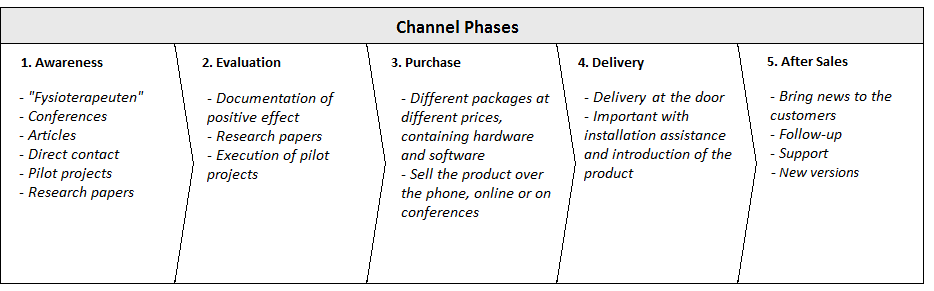
\includegraphics[angle=90,scale=0.7]{channels}
\caption[Channels]{The 5 Channel Phases [modified from \cite{osterwalder}\cite{osterwalderthesis}]}
\end{center}
\end{figure}
\emph{Awareness:} \\ 
We will look into how Cyberlab can raise awareness about the product and how they can get their customers attention.  "Fysioterapeuten" is a magazine targeting physiotherapists in Norway. It is published by \ac{nff} and distributed out to the whole country. "Fysioterapeuten" contains mostly scientific papers, and the idea is that this magazine shall contribute to evolvement of the physiotherapy profession according to the society and populations need. This magazine is read by 9 000 physiotherapists around the country, and articles printed here are seen as scientific and are therefore taken seriously. If Cyberlab could get an article or ad in “Fysioterapeuten” it will contribute to great exposure of the exercise game.  Printing research papers and articles about the exercise game in other credible magazines or newspapers could also get physiotherapists attention.  Taking direct contact with target customers is also a possible solution. This could be done on conferences related to the subject of e.g. technology and health or by visiting physiotherapy clinics. Cyberlab could get the opportunity to present the products and show direct interest in establishing a customer relationship. Physiotherapists see it as very relevant to try a product for an amount of time before they decide to buy. By taking direct contact Cyberlab can introduce a pilot project to the customer, which means testing the product for free in e.g. 6 months. Through conferences, magazines or just word of mouth one can also get an impression of which products that are popular right now. The popularity mark might attract some customers. Physiotherapists working at private clinics do not have the same access to customers as public clinics have, so they might chose to buy a popular product to attract new and more customers. (vet ikke om dette passer under her..)\\ \\ 
(Nav- hjelpemiddelsentralen)\\ \\
\emph{Evaluation:}\\
Physiotherapists points out two very important aspects in evaluating a product. These two are; documented effect of the product and own experience by testing the product. If a physiotherapist should even think about trying the product, it is necessary to provide research papers or statistics that shows positive effect in this kind of games. Documentation will give them a security in the choice of buying the product. (Merkelig setning??) Other physiotherapists providing positive feedback after trying the game also contributes to this security. Another part of the evaluation is by letting physiotherapist be part of pilot projects for a period of time. Then they will have the possibility to test, experience and evaluate the product themselves.\\ \\
\emph{Purchase:} \\
Most physiotherapists have already established connections with suppliers. Ordering and buying products are usually done online, but it can also be by phone or when interesting products are discovered on conferences. Going to the store to buy products is very unusual. But what will physiotherapists buy from Cyberlab? To play this game you need an Xbox Kinect and the exercise game. It is unreasonable to think that a physiotherapist already owns an Xbox Kinect, so the best strategy for Cyberlab would be to sell packages containing both hardware and software.  Packages should include various agreements with appropriate pricing. Some examples are selling the package with or without installation assistance and introduction to the product, or by selling a license agreement and "give away" the package for free.\\ \\
\emph{Delivery:}\\
When buying a new product, especially technical products, there is a need for introduction to the product and maybe also installation assistance. Feedback from interviews with physiotherapists shows the huge importance of start-up help. With much to do at work already, physiotherapists do not have time to pick up deliveries at the postal office, or to setup and learn a new product all by themselves. Buying, receiving, installing and learning should not be difficult or time consuming. The product should be delivered at the door, by someone who can install the product and teach the physiotherapists how to use it.\\ \\
\emph{After sales:}\\
When taking a new product in to use, it is important for physiotherapist to have the possibility to come with feedback. Therefore, Cyberlab should have some kind of support that can take these feedbacks into consideration. Feedbacks can be comments on direct errors or directions on how to make the exercise game more suitable for its use. Cyberlab should follow their customer in the process of learning, and they should inform them of new features and improvements.  
\subsection{Customer Relationships}
Customer relationship is an important part of the customer experience, and it describes what kind of relationship the company establishes with the customers. Support, follow-up and feedback handling are some aspects in establishing customer relationship. Cyberlab has to be available when the customers has problems and needs help. When using a new product one may discover errors or find the product not suitable for its use, so many physiotherapists have an eager to provide feedback on this. Cyberlab should handle these feedbacks, fix errors as soon as possible and take comments on improvements into consideration. Using feedback to make a better product shows customers that Cyberlab takes their comments seriously.  In addition, the customers will hopefully get a more suitable product. The maintenance of a direct and personal contact with the customer shows interest in the use and the experience of the product. All this can contribute to a good customer relationship. Cyberlab should also give their customers a heads ups on updates, new features or products.
\section{Infrastructure Management}
This section is about how Cyberlab creates value. What resources needed and what activities that have to be preformed are described here, as well as if they will get them in-house or from a partner. 

\subsection{Key Resources}

In this section we will describe all the resources needed to make the business model work. The resources are divided into 4 different types, described in table \ref{tab:Resources}.
\newpage

\begin{table}
\centering
    \begin{tabular}{|l|l|}
        \hline
       \textbf{Type of Resource} & \textbf{Resource}  \\ \hline
       \emph{Intellectual} & Insight and experience with fall problematic in elderly \\ \cline{2-2}
        & Programming skills \\ \cline{2-2}
	 	& Creativity \\ \hline
	   \emph{Physical} & Premises \\ \cline{2-2}
	   	& Equipments, i.e. desks and computers \\ \cline{2-2}
	   	& Microsoft Xbox HW \\ \cline{2-2}
	   	& Working Environment \\ \cline{2-2}
	   	& Internet Connections \\ \hline
	   \emph{Human} & System Developers, i.e. programmers and interaction designers \\ \cline{2-2}
	   	& Administration, i.e. marketers, customer related tasks \\ \cline{2-2}
	   	& Support Person(s) \\ \hline
	   \emph{Financial} & The European Union \\
        \hline
    \end{tabular}
    \caption[Resources]{Different types of resources}
    \label{tab:Resources}
\end{table} 
\emph{Intellectual} \\ The developers needs insight and knowledge about different exercises that will strengthen muscles and improve balance in elderly. A thorough background study and research have to be conducted to acquire this knowledge. When they have enough knowledge to form the foundation of an exercise program, they can start to get creative. Creativity is needed to make the game entertaining and easy to understand and conduct. In addition, good programming competencies is needed to develop the game. To make it as cost-efficient as possible, an experienced team should be put together. \\ \\
\emph{Physical} \\ To be able to conduct this project, the team need premises with everything that comes with it, like desks, chairs, computer, internet connection, light etc. Cyberlab is an already established business, so we can assume they already have these premises and equipments established. For this project, they will need specific hardware. The hardware consists of Xbox 360 console and Kinect sensor. In addition an environment where the game can be developed is needed. \\ \\
\emph{Human} \\ Programming skills and creativity are already described above as intellectual resources. So system developers and interaction designers are needed. An administration is needed for marketing, customer related tasks and resource management. When the game is finished it needs to be operated and maintained. These tasks can be done by one or more of the system developers. \\ \\
\emph{Finance} \\ This project is financed by the European Union. 
\subsection{Key Activities}
The game can be described as a Value Chain, which means transforming inputs to a final product. From the knowledge and experience they have acquired the company wants to make a product as good and price-competitive so that their customers would choose their product instead of a product with similar value. A description of the different stages in the value chain is depicted in figure \ref{fig:ValueChainCase}. In some way it can also be thought of as kind of a Value Shop, because they are in some way solving a problem for a specific customer segment. To do this, they will work in an iterative way, where they will have to test and evaluate the game during the development process. The users have to be involved during the development. 
Activities that need to be done include research, development, testing, maintenance and updates, support, marketing and administrative tasks. 

\begin{figure}
\label{fig:ValueChainCase}
\begin{center}
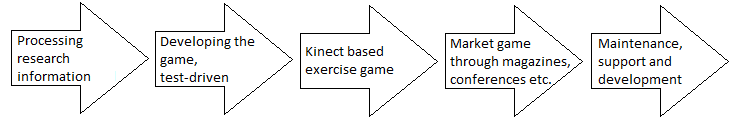
\includegraphics[scale=0.7]{valuechaincase}
\caption[Value Chain for the Kinect Based Exercise Game]{Value chain for the Kinect based exercise game [modified from \cite{osterwalderthesis}]}
\end{center}
\end{figure}
\newpage

\subsection{Key Partnerships}
The main partner in this project is the partnership with Microsoft Xbox. There are several reasons for this. First of all, they need the approvement that they are allowed to develop games for their video game console, and second, they need Microsoft Xbox’ hardware and development environment. They will also have to form an agreement with Microsoft Xbox on how they can sell the product. \\ \\ As mentioned in the introduction, this project is a collaboration between many different entities, where Norut, a national research group, is one of them. Their job in this project is to provide Cyberlab with research. \\ \\ Physiotherapists are their customer segment, but they can also serve as a partner. Becoming partners with different clinics, will make the the marketing and selling easier, because then the actual customer believes in it. \\ \\ If professionals, physiotherapists believes in this, then the government should believe in it. Getting this game into a medical program financed by the government will make this game very credible for the end user. The government could then provide the game to hospitals, care centers, physiotherapy clinics, training groups, and for special cases, when the elderly for example need the game in their own house. \\ \\ This game can fit well into "Samhandlingsreformen", described in chapter 5. We see this games potential as a too for "everyday rehabilitation" (See chapter 5). This require a collaboration between Cyberlab, physiotherapists and the government. Becoming partners with the Norwegian government will first require that the physiotherapists believes in it, so they will first have to join the team. But it is not a requirement that physiotherapists become a partner. However, some kind of collaboration has to be established with the physiotherapists, since they serve as the professionals. This will typically happen in the research, - development -and testing phase.  \\ \\ Having the Norwegian government as a partner will solve some of the financial issues. Most hospitals, physiotherapy clinics and training groups are managed and financed by the government. With them believing in the game and including it as a helping tool that will prolong and improve elderly's life it will be easier to hit the target users. 
\section{Financial Aspects}
In this section all the outgoing and incoming money will be described. All the previous blocks described are contributing to a cost or an income. We will try to provide an as realistic and detailed estimate of both costs and income.
\subsection{Revenue Streams}
The revenue stream describes how the company can earn money, and for Cyberlab this involves selling a product package consisting of the Microsoft Kinect sensor and the exercise game. There are various ways to sell this product, and we will present two solutions.\\ \\
Before pricing the product it is necessary to observe todays market with possible target customers, prices on existing games and physiotherapy tools, and the potential demand for this product. Calculating an exact demand for this product is almost impossible due to the lack of existing games in the same genre for this purpose, and also since the game Cyberlab are going to sell don’t exist yet. In this section we will assume that the exercise game has been made, testet and that it has received a great amount of positive feedback. Physiotherapists in Trondheim has started to use the exercise game, and it’s being appreciated at the same level as other tool used at the clinic. \\ \\ 
Pricing this product depend on existing games and tools, and development cost in hope of achieving a non-negative profit for Cyberlab. We can start by looking at existing products. Cyberlabs exercise game falls under two definitions, a video game and a tool used in physiotherapy for training and rehabilitation. The video game market today exist of a huge amount of various games. They are mostly in affordable price range, where e.g. Nintendo Wii games are priced between 99 - 249 NOK and Xbox Kinect games are priced between 199 - 499. Physiotherapy tools has more variation in price range as the definition of this tools are quite wide. Prices can vary from a fixed price of 75 NOK for a stretch pulley (http://www.ilenfysioterapi.no/priser/)  to 11 000 NOK per month for shockwave therapy leasing (see appendix “Intervju med Nina”). As we will present later, a package consisting of hardware and and Cyberlabs’ exercise game will have a much higher price than other video games on the market. Trying to sell the exercise game for more than the already existing ones will be difficult, so it is therefore highly important for Cyberlab to promote their product as more than just a regular game to justify the price difference. This should be done by emphasizing the products value propositions, which relates the product more to physiotherapy equipment than “just” a video game. \\ \\
Cyberlabs’ market potential, which is also important for setting a suitable price, can be roughly calculated by looking at the number of public and private physiotherapy clinics with support from the government. We looked at four municipalities in Norway, Oslo, Trondheim, Fredrikstad and T{ø}nsberg, where we for each found the number of clinics and compared that number to the population in each municipality. The average ratio we got describe inhabitants per clinic in Norway. Multiplying this with the total population in Norway gave us an approximation of physiotherapy clinics suitable for Cyberlabs’ customer segment. Our calculation (see Appendix blabla for details) shows that Cyberlab has a possible market in approximately 1 200 physiotherapy clinics. \\ \\
We will now present two different solution for how Cyberlab can sell their product, with suitable prices for each solution.  
\begin{table}
\centering
    \begin{tabular}{|l|l|}
        \hline
       \textbf{Package example} & \textbf{Price example}  \\ \hline
       Only the package & 4 000 NOK \\ \hline
	   Package with delivery, installation and introduction & 8 000 NOK \\ \hline
	   Package as a license agreement & 9 500 NOK\\ \hline
	   Package as a license agreement with delivery, \\ 
	   installation and introduction & 13 500 NOK \\
        \hline
    \end{tabular}
    \caption[Priceexample]{A price example}
    \label{tab:Priceexample}
\end{table} 

\subsection{Cost Structure}
Cost structure takes into account all elements that generates costs specific to this game. Cyberlab is an already established business and we can therefore assume that there are not any additional costs associated with premises and some of the "regular" equipments (e.g. Desks, chairs, computers etc.). First we distinguish between fixed and variable costs, investment costs and ongoing costs. Variable costs are associated with demand. In this case it is hard to say anything about the demand and therefore it is hard to say anything about variable costs. In this specific case variable costs will be salaries associated with support, maintenance, marketing and sales. However, since we are dealing with a market which is very hard to analyse with respect to demand, we will make a prediction on how much work is required for each of this tasks. In this way this cost will look more like fixed costs.  \\ \\
In this case fixed costs are associated with salaries to all the involved workers on this project. This includes project manager, developers, researchers and interaction designers. In addition we will also take into account support, marketing and sales, with predicted workload. There are additional costs associated to having an employee, explained shortly.  We define these as fixed costs because the employers are hired to do this job over a fixed period of time. The investment costs associated to this project is the hardware and software needed to develop the game. Other fixed costs include hardware and software that are needed to develop the game. This includes specific hardware and a SDK for the sensor. The commercial price for the Kinect sensor is 1790 NOK \cite{pricekinect}, and the SDK for the sensor is free. In addition they should have a screen for testing purposes. The screen should be big, so we suggest they invest in a projector and 90" projector screen, which should be sufficient for its purpose. We found that the cost of an average screen lies around 895 NOK and 2449 NOK for a projector \cite{priceprojector}\cite{pricescreen}.  Cyberlab has estimated that for developing this game they need a full-time equivalent (FTE) = 1.0, meaning that the workload is equivalent to one person working full time for a year. We assume that this will cover development, testing and administrative tasks. In addition to that, Norut who provides research has also assigned a FTE=1. How many people assigned to the project is unknown and also irrelevant for the cost prediction, (assuming each employee has the same salary). We have done a rough estimate on how much the cost of having FTE = 1 in the private sector is. From \cite{tekna} we found statistics of salary in the private sector in Norway. Assuming that the "average" employer on this project graduated in the end of the 90's, we look at an average gross salary of approximately 730 000 NOK a year. From this we can calculate the average cost of a FTE = 1.0, based on \cite{altinn}, see Table \ref{tab:costofFTE}, which will be 1 003 349 NOK. We did the same calculations for researchers in the government controlled sector and for marketers in the private sector. They both ended up on a cost of 715 577. See appendix for calculations. \\ \\

\begin{table}
\centering
    \begin{tabular}{|l|l|l|l|}
        \hline
       1&Gross Salary & & 730 000 NOK \\ \hline
       2&Holiday Pay & 12.1\% of 1  & 88 330 NOK \\ \hline
	   3&Employee Fee & 14.1\% of 1+2  & 115 385 NOK \\ \hline
	   4&Pension Costs & 8.0 \% of 1 & 58 400 NOK\\ \hline
	   5&Employee Fee of Pension Costs & 14.1\% of 4 & 8 234 NOK \\ \hline
	   6&Insurance & & 2 000 NOK \\ \hline
	   7&Mobile and Internet & & 1 000 NOK \\ \hline
	   & \textbf{SUM} & & \textbf{1 003 349 NOK} \\
	    \hline
    \end{tabular}
    \caption[Cost of FTE = 1]{The cost of FTE = 1 in the private sector}
    \label{tab:costofFTE}
\end{table} 
We will now look as some ongoing costs on a per year basis. The game has to be operated on a server. This can be on a local server located in Cyberlab’s office, a server located at one of the physiotherapy clinics or on a cloud hosted server. The size of a Kinect game varies a lot, depending on quality, colors, how many levels etc. What we do know is that the game will be of fixed size. The dynamic part of the space needed on the server is associated with how many customer profiles it needs to store. This is a hard task to answer, but we assume that the user profiles do not take up that much space, and that Cyberlab can make it with a small server with fixed space. At this stage it is also hard to make an exact assumption on how big the game will become, but from already existing Kinect games, we can assume that the size will not be bigger that 10 GB. From Gogrid Servers \cite{priceserver} we found a small server with storage space of 25 GB. We believe this will be sufficient for Cyberspace's purpose. There is also reasonable to believe that Cyberlab has some space available on their servers. However, if they would have to rent this kind of server space, we are looking at an annual price of \$181.25 which is is roughly 1 087 NOK (with a currency of \$1 = 6 NOK). With new software and technology there will always be some errors and bugs after the product or service’s delivery. We can assume that the first six months are the most critical months, and will require a FTE = 1/4. The remaining life time will only need support for some minor problems that might appear (E.g. customer service, operating the server). This period will require a FTE = 1/8. This is very hard predictable numbers, because this may vary over time, but we look at the different numbers as reasonable average numbers, that take unexpected events into account. With the rapid evolution of technology, it is reasonable to believe that Cyberlab will offer this game for no longer than five years (FINN KILDE PÅ DETTE, before they will have to make new versions. New versions may even be developed during these five years. We do not take the development of new versions into account in our calculation, and we will set the lifetime of this game to be 5 years. \\ \\
Marketing is one of the most important part of selling a product or service. This is especially important in the first year of the games life time. The cost of marketing is difficult to analyse because it depends on how long it will take to acquire customers. A new product or services need to acquire customers quickly, and therefore more resources need to be put into the marketing tasks. We can look at the exercise game as a niche product that is targeting a specific customer segment. Thus, the marketing task needs to be customized for this specific customer segment. When a critical mass (the number of customers needed to survive economically in the market) is reached the market will somehow be self-supported \cite{informationrules}. Thus, the marketing cost will be rather low, and constant. We assume that the first year right before, during and after the release, the marketing task will contribute to a FTE of 1/2. We assume that after being on the market for one year, the customer base should have reached critical mass.  We believe that in a community like this (the physiotherapist community), words spread really fast, and if the game has proved to be good and other physiotherapists are using it, more physiotherapist will most likely buy the game. Even after critical mass is reached, there will still be some marketing related tasks (e.g. keep up with the market, look for new customer segments), so we suggest that the marketing tasks should contribute to a FTE = 1/5 after the first year. With this low workload, Cyberlab should consider to hire a marketing consultant in stead of having a permanent employee. FINNE NOEN TALL PÅ Å LEIE MARKEDSFØRER.\\ \\
As mentioned earlier we suggest that Cyberlab should run pilot projects to document the effect of the game. This will also serve as a very effective way of marketing the game. We suggest that the pilot project should be carried out in two different clinics in Trondheim for convenience, and that it should run for six month. The effect should be documented during the project and after. This documentation should be published in scientific articles and distributed to physiotherapists. (Lurer på om også offentlige klinikker må ha penger for dette? det er vel de som skal dokumentere effekt osv. Vil jo gi de ekstra arbeid.). We assume that the development of the game will take about six months, so the first year will contain the development phase and the pilot project. The pilot project will most likely provide Cyberlab with valueable feedback on the game, where they can both test the usability in a real environment as well as discover bugs and errors. This will require close monitoring from Cyberlab, so we suggest that this will require a FTE = 1/5 for this six months (This equals FTE =1/10). Spending six months on the initial developing and six months on the pilot project, means that Cyberlab is looking at a whole year without revenue. \\ \\
As suggested from our interviews with physiotherapists, Cyberlab should offer their customers help with installation and introductory to the game. This might be a hard job to realize if Cyberlab is to deliver this game to every physiotherapy clinic in Norway. It is not realistic that an employer from Cyberlab will travel to the other side of the country as soon as an clinic order the game. In the first year, we suggest that Cyberlab focus on delivering the game to clinics in Trondheim. Selling the game in only Trondheim to an acceptable price, will not make profit. We believe that Cyberlab is looking at some years before they will make profit. The physiotherapy community is a small community with a lot in common. By the time this game has become well-known in Trondheim, the game has probably got attention from clinics in other cities as well. We suggest that Cyberlab hire some of the physiotherapists that are already using the game to present it on conferences and learn other physiotherapist. In this way, the game will be both more believable to other physiotherapists, as well as Cyberlab do not need to do the hazel with travel around promoting their game.